\chapter{Framework cross-platform mobiele applicatie}
\label{ch:frameworkcrossplatformapp}
\section{Twee grote categorieën}
Ter voorbereiding van het vergelijkende onderzoek tussen de cross-platform mobiele applicatie en de
responsive website, is er voor beide mogelijke manier gezocht om deze vormen van applicaties te ontwikkelen. Voor de cross-platforme
mobiele applicatie zijn deze mogelijke vormen een methode die zeer sterk aansluit bij het ontwikkelen van html-website.
Hierbij wordt de html code in combinatie met css voor de opmaak en JavaScript voor de logica door de compiler omgezet naar een cross-
plaforme mobiele applicatie. Op deze laatste manier wordt er gedurende dit werk niet verder op ingegaan.

\label{sec:architectuurvandecrossplatformemobieleapplicatie}
\section{Architectuur van de cross-platform mobiele applicatie}
Voor de opbouw van de cross-platform mobiele applicatie is geopteerd om te kiezen voor een architectuur waarbij men zoveel mogelijk
code gemeenschappelijk kan hergebruiken. Concreet houdt dit in de men in het Shared-project zowel de definitie van de domeinklassen,
als de code die verantwoordelijk is voor het ophalen van de data uit de REST-service en de mapping definieërt.

De schematische voorstelling van de architectuur van de cross-platform mobiele applicatie ziet er schematisch als volgt uit:
\begin{figure}[ht!]
\centering
\caption{Architectuur van de cross-platforme mobiele applicatie \cite{joshholmes2017}}
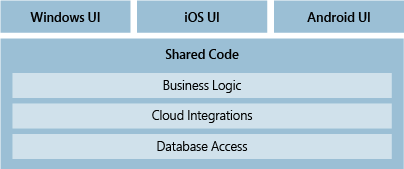
\includegraphics[width=90mm]{./img/architecture.png}
\end{figure}

Voor deze authenticatie in te implementeren, werd er volgend voorbeeld van \cite{authenticatemvcapplication2017} gevolgd.
Eerst werd het voorbeeld aangepast om authenticatie aan de hand van Active Directory te voorzien, maar dit is later terug verwijderd.
Dit omdat het op een externe locatie niet mogelijk is om verbinding te maken met het netwerk waarop deze Active Directory zich bevindt.
De REST-service is dus zodanig opgebouwd dat de gebruikersgegevens niet worden gevalideerd, maar er wel een token teruggegeven wordt door de REST-service.
Verder is deze token wel verplicht toe te voegen aan elke request die gestuurd wordt om data op te vragen.

\label{sec:voordelenvandegekozenapparchitectuur}
\section{Voordelen van de gekozen architectuur}
\subsection{Ontwikkeling en project structuur}
De grote voordelen van de architectuur van de cross-platform mobiele applicatie zijn: Specifieke deelprojecten voor de afzonderlijke
mobiele besturingssystemen en het gemeenschappelijk stellen van bepaalde delen van de programmacode. Dit biedt voor de ontwikkelaar
als pluspunt dat binnen de gekozen ontwikkelomgeving, nl. Visual Studio, dat de oorspronkelijke project-structuur behouden blijft.

Deze manier van werken vereenvoudigt de overstap van de oorspronkelijke ontwikkelingomgevingen, nl. Android Studio voor Android en xcode voor iOS, naar Visual Studio.
Ook de syntax van de code van de deelprojecten werd hierbij overgenomen en vertaald naar C\#.

\subsection{Veiligheid}
Nog een punt waar de mobiele applicatie beter op scoort in vergelijking met de responsive website, is de beveiliging aan de hand van biometrie \footnote{Biometrie wordt gedefinieërd als de wetenschap die gebruikt maakt van biologische lichaamskenmerken om een persoon te identificiëren. \citep{davidcheklingngoandrewbengjinteohjiankunhu2015}}


\subsection{User Interface}
Voor het definiëren van de user interface heeft Microsoft besloten om de bestaande manier van werken over te nemen van de oorspronkelijke platformen, nl. Android, iOS en Universal Windows Platform.
Dit brengt voor de ontwikkelaar zowel een voor- als nadeel met zich mee. Het heeft als voordeel dat, indien men reeds mobiele applicatie voor Android, iOS en windowsphone kan ontwikkelen, men geen
nieuwe opmaaktaal voor de user interface dient aan te leren. Het grote nadeel van deze manier is dat men 3 keer een UI moet definiëren,
dit moet behorende code-behind voor het opvangen van de events uit de UI.

\label{sec:nadelenvandegekozenapparchitectuur}
\section{Nadelen van de gekozen architectuur}
\subsection{User Interface}
Zoals eerder vermeld, brengt het gebruik van de standaard-methodologie van de 3 mobiele platformen een grotere hoeveelheid
werk voor de ontwikkelaar met zich mee. Dit omdat Android, iOS en windowsphone elk hun eigen manier van UI te definiëren en deze niet hergebruikt kan worden.

Voor het opvangen van de events van de UI kan men wel opteren om in de architectuur een facade \footnote{Fasade Design Pattern \cite{dofactorycom2017}} te voorzien, waarnaar de oproepen van events uit de user interface gedelegeerd worden naar de facade.

Op deze manier beperkt de code in de klassen die de events van de user interface opvangen tot het strikt noodzakelijke.
\label{sec:appkosten}
\subsection{Kosten}
De ontwikkeling van een cross-platform mobiele applicatie is een project waaraan de nodige kosten verbonden zijn.
Hieronder volgt een oplijsten van de kosten per fase in het softwareontwikkelingsproces.

\subsubsection{Kosten voor de ontwikkeling}
Reeds bij de ontwikkeling van de cross-platform mobiele applicatie zijn er mogelijks kosten. Zo dient men een licentie op een ontwikkelomgeving
aan de schaffen. Indien men de ontwikkelomgeving kiest die voor dit onderzoek gebruikt werd, nl. Visual Studio 2015 Professional,
komt dit momenteel 499 dollar of 446,7 Euro.

\subsubsection{Kosten voor testen}
Voor een applicatie in de applicatiewinkel van een mobiel besturingssysteem terecht komt, dient deze eerst uitvoerig getest te
worden. Op deze manier worden de mogelijke fouten uit de software gehaald. Fouten in de applicatie kunnen ervoor zorgen dat de applicatie
onverwacht beeïndigd wordt of vastloopt.
Dit beeïndigen of vastlopen kan tot gevolg hebben dat de applicatie slechte reviews krijgt in de applicatiewinkels en bijgevolg minder downloads en inkomsten voor de ontwikkelaar oplevert.

Het testen van de applicatie kan op 2 manieren gebeuren: via een emulator of via een fysiek toestel. Indien men enkel in de emulatoren test, zijn er geen extra kosten aan de testfase van het eindproduct.
Wenst men toch op fysieke toestellen te testen, moet de aankoopkost van deze toestellen ook in rekening worden gebracht.
\newpage
Indien men ervoor kiest om voor de drie grote platformen te ontwikkelen, heeft men naast de kost van de licentie voor Visual Studio of een ander ontwikkelomgeving,
ook de kost van een computer waar het besturingssysteem macOS op geïnstalleerd is in combinatie met Xcode, de ontwikkelomgeving van \cite{xcodemacappstore2017}.
Xcode is een IDE \footnote{Integrated Develop Environment} waarin men applicatie kan ontwikkelen voor iOS, macOS, tvOS en watchOS, de besturingssytemen voor respectievelijk iPhone en iPad,
iMac en de macbook in alle versie, de Apple TV en de Apple Watch. De ontwikkelomgeving is gratis beschikbaar de App Store in macOS .

\subsubsection{Kosten voor publicatie}
Men heeft echter wel nog kennis nodig heeft van Android, iOS en windowsphone om deze applicatie te
kunnen ontwikkelen. Zo moeten er nog steeds 3 applicaties ontwikkeld worden, hetzij wel in een afgeslankte versie.
Dit in tegenstelling tot de responsive webapplicatie waarbij men slechts 1 keer de gebruikersinterface dient te definiëren.

Verder dient ook men de applicatie voor elk mobiel besturingssysteem te publiceren in de appstores van de verschillende
mobiele besturingssystemen. Hieraan zijn  eenmalige of jaarlijkse kosten aan verbonden. Zo dient men voor de publicatie in de App Store van Apple zich eerst inschrijven voor het
Apple Developer Program \citep{appledeveloperprograms2017} . Deze inschrijving kost 99 Amerikaanse dollar per jaar. Verder kunnen bedrijven of organisaties
zich hier ook bij aansluiten, om zo meerdere ontwikkelaars aan te laten sluiten op 1 ontwikkelaarsaccount voor de App Store.
Dit verlaagt de kosten.

Voor Android dient men bij de publicatie van de app \citep{getstartedwithpublishingandroiddevelopers2017} eenmalig 25 Amerikaanse dollar (22,35 Euro) betalen voor de inschrijving.
Verder kan men aan de hand van Developer Console het aantal downloads van de app, het aantal gerapporteerde crashes en de gemiddelde rating die de gebruikers gaven bekijken.
Aan de hand van de recensies die de gebruikers op de app, kan de ontwikkelaar de feedback met eventuele verbeterpunten bekijken.

Indien men de applicatie wenst te publiceren in de 'Microsoft Marcketplaces' van \cite{registerasanappdeveloper2017}
 zoals de Windows Store, Office Store, Azure Marketplaces en nog meer aan te kondigen winkels, dient men voor een individueel account
 eenmalig ongeveer 19 Amerikaarse dollar (16,98 Euro) te betalen aan Microsoft. Voor bedrijfsaccounts komt deze kost neer op +/- 99 dollar (88,50 Euro).

Naast de publicaties van de applicaties, dient de REST-api ook gehost moet worden. Indien men dit in Azure wenst dit doen, komt men op volgende prijsberekening \footnote{App Service bevat 1 core, 1.75 GB RAM en 10 GB opslag.} \footnote{Deze prijzen zijn vermeld in Euro.}.

\addcontentsline{lot}{table}{Uitgewerkte prijsberekening voor hosting van een REST api op Azure \citep{pricingcalculormicrosoftazure2017}}
\begin{flushleft}
  \description{Uitgewerkte prijsberekening voor hosting op Azure}
  \newline
  \begin{tabular}{ | l | l | l | l |}
  \hline
  Omschrijving & Region & Prijscategorie & Prijs (€)
  \\ \hline
  App Service & West-Europa & Basis & 47,06
  \\ \hline
  SQL Database (Single Database) & West-Europa & Basis & 4,20
  \\ \hline
  API management & West-Europa & Standaard & 41,30
  \\ \hline
  Support & nvt & nvt & 0,00
  \\ \hline
   & & Totaal & 92,56
  \\ \hline
  \end{tabular}
\end{flushleft}
